\documentclass[twocolumn]{revtex4}
\usepackage{graphics,graphicx,epsfig,amsmath,multirow,gensymb,commath,textcomp,natbib,blindtext,mhchem,tabularx,array,makecell}
\usepackage[normalem]{ulem}
\newcommand{\squeezeup}{\vspace{-2.5mm}}

\def\bibsection{\section*{\refname}} 
\renewcommand{\thesubsection}{\alph{subsection}}

\renewcommand\theadalign{bc}
\renewcommand\theadfont{\bfseries}
\renewcommand\theadgape{\Gape[4pt]}
\renewcommand\cellgape{\Gape[4pt]}

\begin{document}

\textheight=26.385cm
%Change textheight as the last resort...

\title{Producing light curves for supernova explosions and their usage in determining a value for Hubble's Constant}
 
\author{Jacky Cao, AstroLabs, Lab Partner: Duncan Middlemiss \\ Dates of experiment: 19/10/2017 to 17/03/2017, Date of report: 19/03/2017}

\begin{abstract}              
We have measured the magnitude of supernova explosions over an extended period of 47 days using $0.5$ m and $?.?$ m telescopes situated in Durham and La Palma. We have plotted several light curves and identified Type Ia, Type II, and ?? supernovae. Our fittings have had $\chi^2$ analysis has performed, and it has produced values of ?, ?, ?. We expect our biggest source of uncertainty arose due to the conditions and data analysis that we performed. Using a Type Ia supernova of brightness $00.00$ mag, we have managed to produce a value for Hubble's Constant, $H_0 = 74$ kms$^{-1}$ Mpc$^{-1}$. We attempted to calculate Einstein's coefficient, $\Lambda$, but this was unsuccesful due to redsjhift of something.
\end{abstract}

\maketitle

\vspace{-3ex}
\section{Introduction} 
\vspace{-2ex}

In astronomy, one of the most violent and luminous events which can occur is a supernova explosion. At the end of a massive star's lifetime, there is a possibility that the equilibrium configurations for a star will cease to exist after it has ran out of nuclear fuel to burn. This eventually leads to the final explosion, the luminosity of which when at it's peak can be as bright as a small galaxy \cite{longair}.

Observing these events and measuring their magnitude over a period of time allows us to then plot light curves (magnitude is displayed as a function of time). From visualising this evolution we can draw the conclusion that there is some order in the explosions - they can be grouped together into multiple types as their light curves have similar shapes and features.

Once we have our different groups we can then use them in cosmology for example. One type of supernova explosion called Type Ia's can be used in calculations which leads to a value for Hubble's Constant. The methodology of which will be discussed later in section \ref{appcosmo}.

In studying and using supernovae as a tool, we must understand the underlying physics which creates these awesome cosmic events. (??)

\vspace{-3ex}
\subsection{Supernovae Classification}
\vspace{-2ex}
The two basic classifications for supernovae are Type I and Type II explosions. The main distinction between them both is that the Type I supernova explosion (SNe) has an absence of the Balmer series of hydrogen in their optical spectrum (at maximum light), and Type II does have this hydrogen feature \cite{mod_ast, longair}. (??) 

In the following sections we will discuss the stages which led to the different types of supernovae. (??)=

With these two groups there are further possible subclassifications. This is possible as there are visible differences their light curves and also in their spectral features \cite{longair}. In Table \ref{sn_classes}, I have highlighted the subtypes which we will explore through experimentation and analysis. (??)

\begin{table}[h!]
\centering
\begin{tabular}{c@{\hskip 20pt}c} 
 \hline
 \textbf{Type} & \textbf{Characteristic} \\ 
 Type Ia		& Si II line at $616.0$ nm \\
 			& \em Type Ib and Type Ic also exist \em \\
 Type IIP 		& Reaches a plateau in it's light curve \\
 Type IIL		& Displays a linear decrease in it's light curve \\
 			& \em Type IIn and Type IIb also exist \em \\
 \hline
\end{tabular}
\caption{Some of the subclassifications of supernova \cite{longair}.}
\label{sn_classes}
\end{table}

\vspace{-3ex}
\subsubsection{Type I Supernovae}
\vspace{-2ex}
In understanding why the optical spectra of Type I supernovae does not contain the Balmer hydrogen features, we must look at the physical composition of the objects. Type I SNe occur with stars which have lost their hydrogen envelopes, either from strong mass-loss from their surface layers, or because they involve the explosion of white dwarfs which lost their hydrogen envelopes when they were formed \cite{longair}. 

It is of interest when performing cosmology that we explore the explosions of white dwarfs, this is contained in one of the subgroups of Type I supernovae, Type Ia.

The general consensus is that presupernova, for Type Ia supernovae, there is a white dwarf within a binary system which accretes matter from a donor star, this can be described as the single degenerate model. However, this is also the initial system for dwarf novae and classical novae, better known together as cataclysmic variables \cite{mod_ast}. They too increase in brightness which can lead to some confusion with supernovae, especially with classical novae as they increase in their brightness by a factor of  $\sim 10^6$ \cite{mod_ast}. [more detail??]

The distinction for supernovae is drawn as the white dwarf will increase in it's mass until it reaches the critical Chandrasekhar mass, $1.4 M_{\odot}$ \cite{posn, longair}. As the material is continually compressed on and in the white dwarf, it is heated to a temperature of $T \geq 10^9$ K \cite{longair}, the fusion of the rich carbon and oxygen core can begin. Thermonuclear energy is released and the white dwarf loses it's electron degeneracy pressure, the object is now gravitationally unstable \cite{longair}. However, this energy that is produced disrupts the star and prevents a total collapse into a neutron star, this disruption leads to a supernova explosion \cite{posn}. 

This white dwarf-comapnion star mechanism has support from spectroscopic observations of Type Ia supernovae at maximum light. We find the spectra has silicon, calcium, magnesium, sulphur and oxygen present. These are elements which are the products for when carbon and oxygen are burned in the nuclear fusion processes of (\ce{^{12}C} + \ce{^{12}C}), and (\ce{^{16}O} + \ce{^{16}O}) \cite{longair}.

From spectral fits, we can calculate the velocities of the ejecta material which have been measured to have a range from a mean value of $5,000$ kms$^{-1}$, to a peak that exceeds $20,000$ kms$^{-1}$ \cite{ia_vel}, approximately $7\%$ of the speed of light. Supernovae are incredibly energetic events with the majority of the explosion energy being converted into kinetic \cite{posn}, these explosions offer us a chance to calculate some fundamental properties of the universe [???].

As this process relies on the Chandrasekhar limit, each Type Ia supernova which occurs will be the same as they would follow the same process of collapsing. They are useful as they  

When plotting their magnitudes against time passed we see that their light curves are generally homogeneous. These objects are the most luminous supernovae known, their absolute magnitudes in the B band are typically $M_B = -19.5 \pm 0.1$ \cite{posn}. Using light curve relationships and models we can determine precisely the magnitudes of very distant SNe, this has allowed astronomers to determine the redshift-distance relation for redshifts high redshift objects ($z>1$). Then, with these calculated values it is then possible to estimate the cosmological parameters $\Omega_0$ and $\Omega_\Lambda$. In doing so, it has been found that using Type Ia SNe has produced agreement with the literature value. so and so (cite paper) have done this and produced values of. 

\vspace{-3ex}
\subsubsection{Type II Supernovae}
\vspace{-2ex}
For a star to end it's life as a Type II supernova explosion, it's core must collapse to produce the enormous amounts of energy that we associate with a SNe. For stars more massive than $8 M_{\odot}$, their post-main-sequence evolution relies on the continual burning of carbon, oxygen, and silicon burning. As this process continues to heat up the core to larger temperatures, photodisintegration will start to occur. Photons have enough energy to breakup heavier elements such as iron (\ce{^{56}_{26}Fe}) and helium (\ce{^{4}_{2}He}), this process is endothermic so energy is removed from the gas that would have created the pressure required to support the core of the star \cite{mod_ast}. 

The free electrons which had been supporting the star through degeneracy pressure are now captured by heavy nuclei and by the protons that were produced through photodisintegration. Through the photodisintegration of iron, and combined with electron capture by other elements, most of the core's support disappears and then the core begins to collapse extremely rapidly. 

\vspace{-3ex}
\subsection{Supernova Discovery}
\vspace{-2ex}

When observing the universe the magnitudes that we observe using our instruments are not 

In discovering supernovae it is important that the search is not focussed on just one part of the sky as there is potential for SNe to occur in any region of the sky. What is required is a survey which covers the entire visible sky, data can then be compared day-to-day and any new objects that appear can be verified to see if it is a new supernova or not. [reference] 

One such survey that employs this is the \em{All-Sky Automated Survey for Supernovae }\em (or ASAS-SN). Their setup (??) involves two stations based in Halekala Observatory in Hawaii, and Cerro Tololo International Observatory in Chile. Together they can produce a survey of the entire visible sky up to a depth of $\sim 17$ mag \cite{asn_lc}.

With this case specifically it has been set so that the data is taken automatically, but it requires humans to go over it. Another method that can be used is to observe a location such as a galactic cluster and do essentially the same method.

In the classification of supernovae and in determining their redshifts, spectroscopic observations are required on the objects after they have been discovered \cite{lascumbres}. While we can use light curves to find the type of a supernova, it is more effective to use their spectra as that will allow us to be more certain [??].

\vspace{-3ex}
\subsection{Application to Cosmology} \label{appcosmo}
\vspace{-2ex}

In discovering supernovae we can calculate the rates at which supernovae occur.

Type Ia supernovae are useful to us as they can be classed as standard candles [cite]. With this we can use them to calculate a value for Hubble's Constant, $H_0$, and thus calculate the expansion rate of the Universe.

asdasd \cite{abs_phil}
\begin{equation}
v = H_0 d, 
\end{equation}
with $v$ as the velocity of the receding object, $H_0$ as the value for Hubble's 
find a reference for this.

\vspace{-3ex}
\subsection{Project Aims}
\vspace{-2ex}

Studying the evolution of the magnitudes of different supernovae will allow us to produce a light curve which can be fitted with known models. Through this we can then discover the type of supernova that we are observing. 

The main focus in our experimentation is attempting to collect the data which would form our light curves. 

Could we confirm the expansion rate of the universe through our observations of supernovae? 

In studying supernovae and their relation to cosmology we have chosen the following for our project aims:
\begin{itemize}
 \item To observe supernovae using telescopes based in Durham and La Palma over an extended period.
 \item To use collected data and then to perform photometry on that data to produce plots of the magnitude shown as a function of time (with uncertainties as well).
 \item To then apply templates/models to our data and evaluate the quality of our data by performing more analysis eg. $\chi^2$ tests.
 \item Then using our data for Type Ia supernovae, we hope to produce a value for $H_0$. With this value we can again attempt to evaluate the quality of our data.
 \item As part of our extension projects we are hoping to:
 \begin{itemize}
  \item Perform a \em{galaxy subtraction }\em so that we are just left with the SN object, and then try and perform photometry again. Noting the differences in values we achieve for our magnitudes.
  \item Attempting to discover a SN by observing galactic clusters - areas which have potentially have a higher chance for SNe to occur in.
 \end{itemize}
\end{itemize}

\vspace{-3ex}
\section{Observations} 
\vspace{-2ex}
\subsection{Data Collection}
\vspace{-2ex}

Observing supernova explosions requires instruments which are sensitive enough to receive the photons which have travelled for vast distances before being recorded. In performing such observations (?) our main equipment are telescopes - they come in a wide variety of configurations and each can produce different results.

In collecting the data for our supernova we used three different types of telescopes. Two of them based in Durham on the Department of Physic's Roof, and one in La Palma. 

As we were observing objects which were faint we required that we either have a large telescope to collect as much light as possible, or have good seeing conditions which allowed us to collect as much light as possible over a large observation time.

\vspace{-3ex}
\subsection{Observations Made}
\vspace{-2ex}

Over a period of (?) days we took images of SNe, however this also depended on the conditions and whether it was worth observing if the seeing was bad e.g. obscured by bad weather.

In making observations there were various factors which required to be known.

In Appendix \ref{objectslog} is detailed all the objects that we chose to view over our experimental period, and in Appendix \ref{obslogs} is a more detailed description of the data that we took.

\vspace{-3ex}
\subsection{Data Analysis}
\vspace{-2ex}

As we collected our supernova day by day we performed various photometry techniques to try and calculate the magnitudes of the explosions. 

Once we had collected our data we then proceeded to perform analysis

Data reduction, what was required, blah blah blah. What was used. Don't say dstack script, say a script was used which allowed us to stack images together.

\vspace{-3ex}
\subsection{Data Uncertainties}
\vspace{-2ex}

Throughout the experiment it was important that we kept in mind the uncertainties which may arise from different areas of the experiment. Quantifying these errors allows us to judge whether the data and fittings that we created were good or not. 

\vspace{-3ex}
\subsection{Final Data}
\vspace{-2ex}

asdasd

\vspace{-3ex}
\section{Analysis}
\vspace{-2ex}
\subsection{Supernovae Models}
\vspace{-2ex}

The fitting of the templates/models to our observations.

\vspace{-3ex}
\subsection{Resuluts}
\vspace{-2ex}

sdfsdfsa

\begin{figure}[!h]
\begin{center}
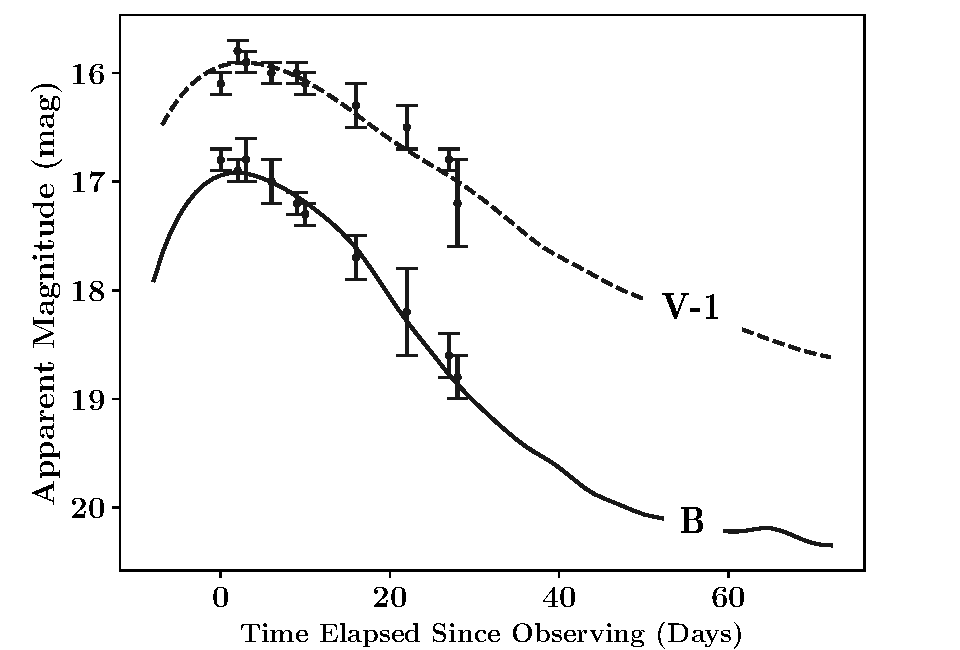
\includegraphics[width=9.5cm]{results/2017hhz}
\caption[]{Intensity maps of four different diffraction patterns taken from different planes: (a) double circle grating in Fourier plane, (b) single circle grating in Fourier plane, (c) L grating in image plane, (d) L grating in `$3f$' plane.}
\label{2017hhz-data}
\end{center}
\end{figure}

\vspace{-3ex}
\section{Discussion}
\vspace{-2ex}

It is highly unlikely that we will see supernova remnants for the supernova that we have been studying, in the shape of the Crab Nebula. Much longer time periods would be required for this. 

[neutrino studying]?

asdasd

\vspace{-5ex}
\section{Conclusions}
\vspace{-2ex}

sdfsdfasdas

\vspace{-5ex}
\section*{Acknowledgements}
\vspace{-2ex}
I would finally like to thank the coffee shops of Durham for putting up with my buy-one-drink-and-stay-in-there-for-six-hours mentality. It has allowed me to complete my lab report in a slightly buzzed but also happy state.


\bibliographystyle{abbrv}
\bibliography{supernovae}

\clearpage
\onecolumngrid
\vspace{-3ex}
\section*{Appendix A - Objects Log} \label{objectslog}
\vspace{-2ex}
A list of the objects that were chosen to be observed, and then the subsequent notes on them. Not all objects were chosen to be observed for an extended period, the ones noted were observed for a couple of nights to ensure suitability. The subsequent observation logs can be found in Appendix B.

{\renewcommand{\arraystretch}{1.2}%
\begin{table}[h!]
\centering    
\begin{tabularx}{\textwidth}{c c c c @{\hskip 5pt} c c X}
    \hline
    \textbf{Object} & \textbf{RA} & \textbf{Dec} & \textbf{Magnitude} &\textbf{First Discovered} &\textbf{Type} & \textbf{Notes} \\ 
    *ASASSN-17mz & 23:56:21.82 & +32:27:24.08 & 14.6 & 2017/09/30.500 & Ia & {Too close to galactic nucleus, cannot see}  \\
    *AT2017hld & 22:18:22.849 & +34:45:08.46 & 16.1 & 2017/10/17.339 & CV & {Cataclysmic Variable, stopped observing}  \\
    *2017hky & 11:23:30.514 & +63:21:59.43 & 16.2 & 2017/10/16.640 & II & {Not viewable from Durham or La Palma}  \\
    2017hhz & 01:44:16.75 & +12:15:18.00 & 16.83 & 2017/10/16.140 & Ia & {A measured redshift, $z=0.0392$}  \\
    AT2017gvb & 08:04:42.34 & +61:31:41.50 & 17.33 & 2017/09/26.59 & unk & {-}  \\
    *ASASSN-17nb & 07:27:37.32 & +35:36:28.30 & 17.31 & 2017/09/25.59 & II & {Object is dwarfed by brightness of the galaxy}  \\
    2017hle & 01:07:36.060 & +32:24:30.00 & 18.0 & 2017/10/18.684 & Ia-91bg & {-}  \\
    2017hou & 04:09:02.140 & -01:09:36.40 & 17.9 & 2017/10/24.370 &Ia & {Viewable from La Palma}  \\
    *AT2017hmw & 01:07:16.570 & +31:25:28.88 & 17.2 & 2017/10/19.415 & CV & {Cataclysmic Variable}  \\
    2017hpa & 04:39:50.750 & +07:03:54.90 & 17.9 & 2017/10/15.346 & Ia & {Viewable from La Palma}  \\
    *AT2017hnm & 01:42:03.24 & +42:31:08.50 & 16.69 & 2017/10/23.44 & unk & {Another star in the image dwarfs the SN in brightness}  \\
    AT2017hpm & 08:04:15.100 & -00:03:58.03 & 16.4 & 2017/10/26.290 & unk & {-}  \\
    *AT2017hqa & 01:08:59.160 & +32:38:04.10 & 17.3 & 2017/10/26.740 & unk & {Unobservable, too close to galactic centre}  \\
    2017hqc & 23:23:08.210 & +10:38:54.63 & 18.0 & 2017/10/27.490 & Ia & {-}  \\
    *AT2017hrr & 11:29:06.490 & -08:59:18.56 & 15.4 & 2017/10/30.607 & unk & {Cannot view from Durham or La Palma}  \\
    *AT2017hhq & 00:42:50.230 & +41:15:27.10 & 17.7 & 2017/10/30.599 & NV & {A nova close to M31}  \\
    AT2017htb & 22:09:38.520 & +17:39:39.56 & 15.7 & 2017/11/02.190 & unk & {-}  \\
    \hline      
\end{tabularx}
\caption{Objects that we chose to observe and notes on them. RA is the Right Ascension, given in units of hours : arcminutes : arcseconds. Dec is the Declination, degrees : minutes : seconds. The stated magnitude is the initial magnitude that the object was discovered in the V band. Objects marked with an asterisk $*$ were objects which we chose to stop observing, the reason provided in the notes.}
\label{objects}
\end{table}


\clearpage

\onecolumngrid
\vspace{-3ex}
\section*{Appendix B - Observation Logs} \label{obslogs}
\vspace{-2ex}
Given below are all the observations which were made during our observation periods. The exposures column is of the following format: ($x: y, z$ s), where $x$ is the band in which the images were taken in, $y$ the number of exposures taken, and $z$ the exposure time which was used, in units of seconds.
{\renewcommand{\arraystretch}{1.2}%
\begin{table}[h!]
\centering    
\begin{tabularx}{\textwidth}{c@{\hskip 5pt} c c@{\hskip 5pt} c@{\hskip 5pt} c@{\hskip 5pt} X}
    \hline
    \textbf{Date} & \textbf{Object} & \textbf{Time} & \textbf{Exposures} & \textbf{  Conditions  } & \textbf{Notes} \\ 
    20/10/17 & 2017hhz & 22:25:34 to 22:58:50 & \makecell{B: 5, 120s \\ V: 5, 120s} & {Clear} & {pt5m: -}  \\
    	& ASASSN-17nb &  02:56:08 to 03:23:36 & \makecell{B: 5, 60s \\ V: 5, 60s} & {Cloudy} & {pt5m: Images produced have a lot of noise.} \\      
	
    21/10/17 & - & - & - & Cloudy & {\em No observations: weather not sufficient in Durham or La Palma for observations. \em} \\
    
    22/10/17 & AT2017hmw &  21:52:20 to 22:31:49 & \makecell{B: 5, 120s \\ V: 5, 120s} & {Clear} & {pt5m: -} \\  
    & 2017hhz & 22:40:20 to 23:19:50 & \makecell{B: 4, 60s \\ V: 12, 60s} & {Clear} & {pt5m: -}  \\
    & ASASSN-17nb &  02:42:45 to 03:10:46 & \makecell{B: 5, 120s \\ V: 5, 60s} & {Clear} & {pt5m: -} \\  
    & AT2017gvb & 03:12:31 to 03:58:58 & \makecell{B: 5, 180s \\ V: 5, 120s} & {Clear} & {pt5m: -} \\    
    
    23/10/17 & 2017hhz & 22:53:12 to 23:32:42 & \makecell{B: 5, 120s \\ V: 5, 120s} & {Cloudy} & {pt5m: Data produced has FWHM ranging from $1.6$ to $9.9$.} \\  
    
    24/10/17 & 2017hhz & 22:44:01 to 23:23:30 & \makecell{B: 5, 120s \\ V: 5, 120s} & {Cloudy} & {pt5m: Data is noisy, potentially another object transited across the frame while observing.} \\  
    
    25/10/17 & - & - & - & {Cloudy} & {\em No observations: too cloudy for observations in Durham, and items in pt5m queue were pushed out in favour of other objects. \em} \\
    
    26/10/17 & 2017hle & 20:54:44 to 21:09:03 & \makecell{B: 4, 60s \\ V: 4, 60s} & {Clear} & {FE16: - }  \\
    & 2017hhz &  21:18:00 to 21:25:31 & \makecell{B: 4, 60s \\ V: 4, 60s} & {Clear} & {FE16: -} \\ 
    & AT2017hmw &  21:29:15 to 21:39:36 & \makecell{B: 4, 60s \\ V: 4, 60s} & {Cloudy} & {FE16: -} \\
    & Messier-7 &  21:50:23 to 21:54:47 & {C: 1, 60s} & {Slightly Cloudy} & {FE16: Test object for SN discovery.} \\
    & Messier-10 &  21:55:47 to 22:00:13 & {C: 1, 60s} & {Cloudy} & {FE16: Test object for SN discovery.} \\
    & AT2017hnm &  23:27:22 to 23:41:55 & \makecell{B: 5, 120s \\ V: 3, 120s} & {Clear} & {pt5m: -} \\ 
    & AT2017gvb &  - & - & {-} & {pt5m: Object pushed out of the queue in favour of others.} \\

    27/10/17 & AT2017hqa & 18:48:12 to 18:52:59 & \makecell{B: 4, 60s} & {Cloudy} & {FE16: Object too close to galactic nucleus. }  \\
    & AT2017hnm &  18:56:34 to 19:00:23 & \makecell{C: 1, 60s} & {Slightly Cloudy} & {FE16: Object too dim, cloud cover reduced light we were receiving.} \\
    & Abell 426 &  19:04:23 to 19:15:41 & \makecell{C: 1, 60s \\ B: 9, 60s \\ V: 9, 60s} & {Clear} & {E14: Object to observe to discover new SN.} \\
    & 2017hhz &  20:11:35 to 20:22:43 & \makecell{B: 4, 60s \\ V: 4, 60s} & {Cloudy and Windy} & {E14: Seeing is bad due to the weather.} \\
    & 2017hle &  20:26:18 to 20:37:35 & \makecell{B: 4, 90s \\ V: 4, 90s} & {Slightly Cloudy} & {E14: Seeing is bad in these images as well.} \\
    & 2017hou &  23:48:09 to 23:50:14 & \makecell{B: 2, 120s} & {-} & {pt5m: Only two frames taken, not sufficient data.} \\
    \hline      
\end{tabularx}
\label{obs_logs1}
\end{table}

{\renewcommand{\arraystretch}{1.2}%
\begin{table}[h!]
\centering    
\begin{tabularx}{\textwidth}{c@{\hskip 5pt} c c@{\hskip 5pt} c@{\hskip 5pt} c@{\hskip 5pt} X}
    \hline
    \textbf{Date} & \textbf{Object} & \textbf{Time} & \textbf{Exposures} & \textbf{  Conditions  } & \textbf{Notes} \\ 
    27/10/17 & AT2017gvb &  02:16:01 to 03:03:05 & \makecell{B: 5, 120s \\ V: 5, 120s} & {Clear/Cloudy} & {pt5m: Some images are more noisy due to clouds.} \\
    
    28/10/17 & AT2017hnm &  21:41:55 to 22:21:25 & \makecell{B: 5, 120s \\ V: 5, 120s} & {Clear} & {pt5m: -} \\
    & 2017hhz &  21:28:50 to 21:30:50 & \makecell{B: 1, 120s} & {Clear} & {pt5m: -} \\
    
    29/10/17 & 2017hle &  21:22:39 to 21:41:21 & \makecell{B: 10, 120s \\ V: 1, 120s} & {Clear} & {pt5m: Mistake on our part to take so many images in B band, and only one in V band.} \\
    & AT2017hnm &  21:55:34 to 22:35:04 & \makecell{B: 5, 120s \\ V: 5, 120s} & {Slightly Cloudy} & {pt5m: -} \\
    & 2017hhz &  23:16:48 to 23:56:18 & \makecell{B: 5, 120s \\ V: 5, 120s} & {Clear} & {pt5m: -} \\
    & 2017hou &  00:33:33 to 01:13:02 & \makecell{B: 5, 120s \\ V: 5, 120s} & {Clear} & {pt5m: -} \\
    & 2017hqc &  01:16:20 to 01:41:20 & \makecell{B: 4, 120s \\ V: 4, 120s} & {Clear} & {pt5m: -} \\
    & AT2017gvb &  02:18:51 to 02:55:47 & \makecell{V: 13, 180s} & {Clear} & {pt5m: Long exposure and large number of exposures chosen as a test to see the quality of stacking them.} \\
    
    30/10/17 & 2017hle &  21:18:56 to 21:58:25 & \makecell{B: 10, 120s \\ V: 10, 120s} & {Clear} & {pt5m: -} \\
    & 2017hhz &  22:06:34 to 22:46:04 & \makecell{B: 5, 120s \\ V: 5, 120s} & {Clear} & {pt5m: -} \\
    & AT2017gvb &  02:04:22 to 03:02:50 & \makecell{V: 20, 180s} & {Clear} & {pt5m: An human error, we re-selected this object from the previous night instead of the one with the correct number of required frames for each band.} \\
    
    31/10/17 & - & - & - & {Cloudy} & {\em No observations: too cloudy for observations in Durham and La Palma. \em} \\
    
    01/11/17 & 2017hle & 23:56:53 to 00:15:35 & \makecell{B: 5, 120s \\ V: 5, 120s} & Clear & {pt5m: -} \\
    & AT2017hnm & 00:18:23 to 00:57:55 & \makecell{B: 5, 120s \\ V: 5, 120s} & Clear & {pt5m: -} \\
    & 2017hhz & 01:00:47 to 01:40:17 & \makecell{B: 5, 120s \\ V: 5, 120s} & Clear & {pt5m: -} \\
    & 2017hou & 01:43:38 to 02:23:08 & \makecell{B: 5, 120s \\ V: 5, 120s} & Clear & {pt5m: -} \\
    
    02/11/17 & - & - & - & {Cloudy} & {\em No observations: too cloudy for observations in Durham and La Palma. \em} \\
    
    03/11/17 & - & - & - & {Cloudy} & {\em No observations: too cloudy for observations in Durham and La Palma. \em} \\
    
    04/11/17 & - & - & - & {Cloudy} & {\em No observations: too cloudy for observations in Durham and La Palma. \em} \\
    
   05/11/17 & ASASSN-17mz & 17:53:45 to 18:09:34 & \makecell{B: 8, 60s \\ V: 8, 60s} & {Clear} & {FE16: -} \\
   & 2017hhz & 18:50:39 to 19:24:43 & \makecell{B: 8, 120s \\ V: 8, 60s} & {Clear} & {FE16: -} \\
   & AT2017htb & 19:38:14 to 20:02:16 & \makecell{B: 8, 60s \\ V: 8, 60s} & {Slightly Cloudy} & {W14: -} \\
   & 2017hle & 20:05:49 to 20:08:28 & \makecell{V: 2, 60s} & {Cloudy} & {W14: Stopped taking exposures after viewing the weather.} \\
   & 2017hqc & 20:14:16 to 20:18:25 & \makecell{V: 3, 60s} & {Cloudy} & {W14: Seeing if images will be strongly affected by the cloud cover.} \\
   & AT2017hhq & 20:33:58 to 20:42:26 & \makecell{B: 4, 60s \\ V: 4, 60s} & {Clear} & {W14: -} \\
       \hline      
\end{tabularx}
\label{obs_logs2}
\end{table}

{\renewcommand{\arraystretch}{1.2}%
\begin{table}[h!]
\centering    
\begin{tabularx}{\textwidth}{c@{\hskip 5pt} c c@{\hskip 5pt} c@{\hskip 5pt} c@{\hskip 5pt} X}
    \hline
    \textbf{Date} & \textbf{Object} & \textbf{Time} & \textbf{Exposures} & \textbf{  Conditions  } & \textbf{Notes} \\ 
    05/11/17 & AT2017hhq & 19:38:14 to 20:02:16 & \makecell{B: 3, 30s \\ V: 3, 30s \\ R: 3, 30s} & {Cloudy} & {E14: Images taken so that we can produce a colour image. } \\
    
    06/11/17 & - & - & - & {Cloudy, and Rain} & {\em No observations: too cloudy for observations in Durham, and torrential rain in La Palma. \em} \\
    
    07/11/17 & - & - & - & {Cloudy and Rain} & {\em No observations: too cloudy for observations in Durham, and torrential rain in La Palma. \em} \\
    
    08/11/17 & - & - & - & {Cloudy and Rain} & {\em No observations: too cloudy for observations in Durham, and torrential rain in La Palma. \em} \\
    
       \hline      
\end{tabularx}
\caption{Observing logs for the entire observation period for our experiment.}
\label{obs_logs3}
\end{table}


\clearpage

\twocolumngrid
\vspace{-3ex}
\section*{Appendix C - Set of Sample Data}
\vspace{-2ex}

\end{document}